\documentclass[thesis=M,english]{FITthesis}[2012/06/26]

\usepackage[utf8]{inputenc}

\usepackage{graphicx}
\usepackage{tabularx}
\usepackage{booktabs}
\usepackage{csvsimple}
\usepackage{rotating}
\usepackage{subcaption}
\usepackage[usenames,dvipsnames]{color}
\usepackage{blindtext}
\usepackage{dirtree}


\newcommand{\myblindtext}{\textcolor{Gray}{\blindtext}}
\newcommand{\myBlindtext}{\textcolor{Gray}{\Blindtext}}
\newcommand{\todo}[1]{\textcolor{red}{[[#1]]}}
\newcommand{\edit}[1]{\textcolor{blue}{#1}}


\department{Department of Computer Systems}
\title{Current development of authenticated encryption and its usage in TLS protocol}
\authorGN{Jan}
\authorFN{Žák}
\authorWithDegrees{Bc. Jan Žák}
\supervisor{prof. Ing. Róbert Lórencz, CSc.}
\acknowledgements{\todo{Acknowledgements}}
\abstractEN{\todo{Summarize the contents and contribution of your work in a few sentences in English language.}}
\abstractCS{\todo{V několika větách shrňte obsah a přínos této práce v českém jazyce.}}
\placeForDeclarationOfAuthenticity{Prague}
\declarationOfAuthenticityOption{4} % TODO
\keywordsCS{\todo{Replace with comma-separated list of keywords in Czech.}}
\keywordsEN{\todo{Replace with comma-separated list of keywords in English.}}


\begin{document}


\begin{introduction}

At its core, the Internet is built on top of IP and TCP protocols, which are used to package data into small packets for transport. As these packets travel across the world, they cross many computer systems in many countries. Because the core protocols don't provide any security by themselves, anyone with access to the communication links can gain full access to the data as well as change the traffic without detection.

Over the last years, the Internet has grown into a major platform for the world's communication. The Internet's trustworthiness has become critical to its success. If a person cannot trust that they are communicating with the party they intend, they won't give out their confidential data. If they cannot be assured that delivered information isn't modified in transit, they won't trust it as much.

The important properties of confidentiality, authentication and integrity are currently best provided on the Internet by the TLS protocol. The HTTP protocol implements it in its secure HTTPS variant, which means using \textit{"https://"} URLs. In the past, websites have deployed HTTPS rarely, often only when financial transactions take place.

More recently, however, it has become apparent that nearly all activity on the Internet can be considered sensitive. If a third party can modify content in transit, the power of the Internet can easily be turned against the user. For example, internet providers can "harmlessly" insert advertisements into websites. More hostile attacks include editing crucial information on the website, or injecting malware.

The TLS protocol does not dictate which cryptographic algorithms need to be used. Instead, TLS serves as a framework establishing and maintaining a secure comminucation channel suitable for sending sensitive messages, while new cryptographic algorithms can be implemented using a common interface.

Currently the TLS protocol uses a MAC-then-Encrypt generic composition to achieve both confidentiality and integrity goals. More recently, the idea of providing both confidentiality and integrity goals using a single cryptosystem has become accepted. In this concept, the combination of encryption and authentication algorithm is replaced by a single authenticated encryption algorithm, such as AES-GCM.

In 2013, CAESAR was announced. It is a worldwide cryptographic competition, focused on finding new methods of authenticated encryption, that offer advantages against commonly used AES-GCM and will be suitable for widespread adoption. Submitted algorithms will be publicly evaluated by committee of researchers in fields of cryptography and cryptoanalysis.



\end{introduction}

\chapter{Transport Layer Security (TLS) protocol}

\begin{figure}[t]
  \centering

  \begin{tikzpicture}
    \node (table) [matrix,row sep=\nodeheight,column sep=\nodewidth] {
      \node {\url{http://google.com}}; & \node {\url{https://google.com}}; \\
      \node (table-layer1) [rect] {HTTP}; & \node (table2-layer1) [rect] {HTTPS}; \\
      & \node (table2-layer2a) [rect] {TLS}; \\
      \node (table-layer2) [rect] {TCP}; & \node (table2-layer2b) [rect] {TCP}; \\
      \node (table-layer3) [rect] {IP}; & \node (table2-layer3) [rect] {IP}; \\
      \node (table-layer4) [rect] {Ethernet}; & \node (table2-layer4) [rect] {Ethernet}; \\
    };

    \node (table2-layer2) [draw,dashed,fit={($(table2-layer2a.north west)+(-0.25*\nodeheight,0.25*\nodeheight)$) ($(table2-layer2b.south east)+(0.25*\nodeheight,-0.25*\nodeheight)$)}] {};

    \node [right=1 of table2-layer1] {\textit{Application Layer}};
    \node [right=1 of table2-layer2b] {\textit{Transport Layer}};
    \node [right=1 of table2-layer3] {\textit{Network Layer}};
    \node [right=1 of table2-layer4] {\textit{Link Layer}};

    \path [line] (table-layer1) -- (table-layer2);
    \path [line] (table-layer2) -- (table-layer3);
    \path [line] (table-layer3) -- (table-layer4);

    \path [line] (table2-layer1) -- (table2-layer2a);
    \path [line] (table2-layer2a) -- (table2-layer2b);
    \path [line] (table2-layer2b) -- (table2-layer3);
    \path [line] (table2-layer3) -- (table2-layer4);

    \path [line,->] ($(table-layer2.east)+(0.5,0)$) -- ($(table2-layer2b.west)+(-0.5,0)$) node[midway,below,align=center] {encryption \\ added};
  \end{tikzpicture}

  \caption{Role of TLS in TCP/IP Reference Model}
  \label{figure/network-model}
\end{figure}


TLS is a security protocol used in almost 100\% of secure Internet transactions. Essentially, TLS transforms a typical reliable transport protocol (such as TCP) into a secure communication channel suitable for sending sensitive messages. TLS does not dictate which cryptographic algorithms need to be used. Instead, TLS serves as a framework establishing and maintaining a secure comminucation channel, while new cryptographic algorithms can be implemented using a common interface.

Adding encryption to an existing protocol is best performed in a transparent way, so that applications using the protocol library do not need to change their code to support encryption. A perfect example is HTTP protocol. A HTTP library can support both plaintext HTTP and encrypted HTTPS, and an application using this library can select the protocol simply in an URL, by specifying \textit{http://} or \textit{https://} respectively. See \autoref{figure/network-model}.

TLS has four main goals, listed here in the order of priority:

\begin{description}
  \item[Cryptographic security] This is the main issue: enable secure communication between any two parties who wish to exchange information.
  \item[Interoperability] Independent programmers should be able to develop programs and libraries that are able to communicate with one another using common cryptographic parameters.
  \item[Extensibility] TLS is effectively a framework for the development and deployment of cryptographic protocols. Its important goal is to be independent of the actual cryptographic primitives (e.g., ciphers and hashing functions) used, allowing migration from one primitive to another without needing to create new protocols.
  \item[Efficiency] The final goal is to achieve all of the previous goals at an acceptable performance costreducing costly cryptographic operations down to the minimum and providing a session caching scheme to avoid them on subsequent connections. \cite{ristic2014bulletproof}
\end{description}

Whereas TLS provides security over reliable TLS communication, there also exists its variant, DTLS protocol. DTLS is deliberately designed to be as similar to TLS as possible, both to minimize new security invention and to maximize the amount of code and infrastructure reuse. \cite{rfc6347} This thesis is about TLS only.

\section{Standardization}

The Internet is the result of a long-term collaboration between governments, academia, and businesses seeking to create a worldwide communication network. For the Internet to function correctly, it must be based upon standardized communication protocols.

Standards concerning the Internet are produced by the Internet Engineering Task Force (IETF) non-profit organization, where experts from around the world collaborates in work groups focused on specific area. IETF produces an informal series of documents known as Requests for Comments (RFCs). For a document to become an Internet standard, it is begins its life by being proposed as an RFC on the standardization track. RFCs in development are temporarily available as \textit{Internet Drafts}. After approval from IETF may be published as \textit{Proposed Standard}. \cite{dent2004user}

There are also other classes of RFCs, most notably experimental and informational RFCs. IETF RFCs cover all the topics of interest to an implementer working with the Internet, which would explain why there are so many of them\footnote{\url{http://www.rfc-editor.org/rfc-index.html}} - over 7400 at the time of writing.

Many of IETF RFCs describe security algorithms, protocols, or recommendations. The most interesting for this thesis are these produced by TLS working group\footnote{\url{https://tools.ietf.org/wg/tls/}}, such as:

\begin{description}
  \item[RFC2246] The TLS Protocol Version 1.0
  \item[RFC4346] The Transport Layer Security (TLS) Protocol Version 1.1
  \item[RFC5246] The Transport Layer Security (TLS) Protocol Version 1.2
  \item[draft-ietf-tls-tls13] The Transport Layer Security (TLS) Protocol Version 1.3 (work in progress)
  \item[RFC5288] AES Galois Counter Mode (GCM) Cipher Suites for TLS
  \item[RFC6655] AES-CCM Cipher Suites for Transport Layer Security (TLS)
\end{description}

TLS implementations are typically written as a set of functions that generate and parse all TLS record messages, and perform the relevant cryptographic operations. The state machine that this process must implement, is currently not standardized, and differs between implementations. Allowing unexpected transitions in this state machine can lead to unexpected behavior. There is an effort to standardize the TLS state machine to allow formal verification of core components in cryptographic protocol libraries. \cite{tls-state-machine}

\section{Records}

\begin{figure}
  \centering

  \begin{tikzpicture}
    \node (row1) [struct] {
      \node (type) [rect,minimum width=1cm] {Type}; & \node (version) [rect,minimum width=2cm] {Version}; & \node (length) [rect,minimum width=2cm] {Length}; \\
    };
    \node (row2) [struct,anchor=north west] at ($(row1.south west)+(1cm,-\nodeheight)$) {
      \node (header) [rect,minimum width=2cm] {Header}; & \node (data) [rect,minimum width=7cm] {Data}; \\
    };

    \path [draw] (row1.south west) -- (header.north west);
    \path [draw] (row1.south east) -- (header.north east);
  \end{tikzpicture}

  \caption{TLS record}
  \label{figure/tls-record}
\end{figure}


At a high level, TLS protocol specifies a structure of every record (packet). Each TLS record starts with a short header, which contains information about the record type (subprotocol), protocol version and data length. Message data follows the header. See \autoref{figure/tls-record} for record structure.

The record type is identified in the record by 1-byte integer ID as specified in \autoref{figure/tls-record-types}. The protocol version can be either SSL 3.0 (deprecated), TLS 1.0, TLS 1.1, TLS 1.2 and it is identified in the record by 2-byte integer ID as specified in \autoref{figure/tls-versions}. The data length field is 2-byte long and it specifies the message data length.

There are the following record types (subprotocols):

\begin{description}
  \item[Handshake protocol] The handshake protocol to negotiate connection parameters, such as the cipher suite, authenticate each other and verify that handhshake messages have not been modified by an attacker.
  \item[ChangeCipherSpec protocol] The ChangeCipherSpec protocol contains a single message, which is a signal from the sending side that it obtained enough information to generate the connection parameters, such as the encryption keys, and is switching all further communication to encryption. Client and server both send this message when the time is right.
  \item[Alert protocol] Alerts are intended to use a simple notification mechanism to inform the other side in the communication of exceptional circumstances. They're generally used for error messages, as listed in \autoref{figure/tls-alert-types}.
  \item[Application protocol] The Application protocol carries application messages, which are just opaque byte arrays as far as TLS is concerned. These messages are packaged, fragmented, and encrypted by the record layer, using the current connection security parameters, such as the negotiated cipher suite.
  \item[Heartbeat protocol] The Heartbeat protocol extension allows a keep-alive functionallity without performing renegotiation. Its purpose is intended especially for DTLS, however it is implemented also in TLS.
\end{description}

This thesis focuses on negotiation of the cipher suite in the Handshake protocol and on application data encryption in the Application protocol.

\section{Handshake protocol}
\label{toc/tls-handshake}

When a client and server start communicating, they use the handshake protocol to negotiate connection parameters, such as the cipher suite, authenticate each other and verify that handhshake messages haven't beed modified by an attacker. It is the most complex part of the TLS protocol, because it performs these tasks:

\begin{itemize}
  \item exchange supported capabilities and agree on shared connection parameters (TLS protocol version, cryptographic algorithms)
  \item exchange necessary cryptographic parameters to agree on shared secret values (\textit{master secret}) using public-key cryptography
  \item exchange certificates or other cryptographic information to authenticate one another
  \item verify that the handshake hasn't beed tampered by a third party
  \item verify that both parties have calculated the same secret values and they can be reliably used to transport application data via record protocol
\end{itemize}

This phase usually takes 6-13 messages (see \autoref{tls-handshake-types} for list of all message types) in 3-4 network flights, depending on which features are used. There can be many variations in the exchange, depending on the configuration and supported protocol extensions. In practice, we can see three common flows:

\begin{itemize}
  \item full handshake with client and server authentication
  \item basic handshake with server authentication
  \item abbreviated handshake that resumes an earlier session
\end{itemize}

\begin{figure}
  \centering

  \begin{tikzpicture}
    \node (table) [matrix,row sep=0.5*\nodeheight,column sep=2.5*\nodewidth] {
      \node (client) [rect] {Client}; & \node (server) [rect] {Server}; \\[0.5*\nodeheight]
      \node (client1) [circle] {1}; & \coordinate (server1); \\
      \coordinate (client2); & \node (server2) [circle] {2}; \\
      \coordinate (client3); & \node (server3) [circle] {3}; \\
      \coordinate (client4); & \node (server4) [circle] {4}; \\
      \coordinate (client5); & \node (server5) [circle] {5}; \\
      \coordinate (client6); & \node (server6) [circle] {6}; \\
      \node (client7) [circle] {7}; & \coordinate (server7); \\
      \node (client8) [circle] {8}; & \coordinate (server8); \\
      \node (client9) [circle] {9}; & \coordinate (server9); \\
      \node (client10) [circle] {10}; & \coordinate (server10); \\
      \node (client11) [circle] {11}; & \coordinate (server11); \\
      \coordinate (client12); & \node (server12) [circle] {12}; \\
      \coordinate (client13); & \node (server13) [circle] {13}; \\[0.5*\nodeheight]
      \coordinate (client13b); & \coordinate (server13b); \\[0.5*\nodeheight]
      \node (client14) [circle] {14}; & \node (server14) [circle] {14}; \\
      \coordinate (client15); & \coordinate (server15); \\
    };

    \begin{pgfonlayer}{bg}
      \path [draw,dashed] (client) -- (client15);
      \path [draw,dashed] (server) -- (server15);
    \end{pgfonlayer}
    \path [line] (client1) -- (server1) node[above,near start] {\textit{ClientHello}};
    \path [line] (server2) -- (client2) node[above,near start] {\textit{ServerHello}};
    \path [line] (server3) -- (client3) node[above,near start] {\textit{Certificate}${}^\ast$};
    \path [line] (server4) -- (client4) node[above,near start] {\textit{ServerKeyExchange}${}^\ast$};
    \path [line] (server5) -- (client5) node[above,near start] {\textit{CertificateRequest}${}^\ast$};
    \path [line] (server6) -- (client6) node[above,near start] {\textit{ServerHelloDone}};
    \path [line] (client7) -- (server7) node[above,near start] {\textit{Certificate}${}^\ast$};
    \path [line] (client8) -- (server8) node[above,near start] {\textit{ClientKeyExchange}};
    \path [line] (client9) -- (server9) node[above,near start] {\textit{CertificateVerify}${}^\ast$};
    \path [line] (client10) -- (server10) node[above,near start] {[\textit{ChangeCipherSpec}]};
    \path [line] (client11) -- (server11) node[above,near start] {\textit{Finished}};
    \path [line] (server12) -- (client12) node[above,near start] {[\textit{ChangeCipherSpec}]};
    \path [line] (server13) -- (client13) node[above,near start] {\textit{Finished}};
    \path [draw] ($(client13b)-(0.5*\nodewidth,0)$) -- ($(server13b)+(0.5*\nodewidth,0)$) node[above,midway] {handshake completed};
    \path [line,<->] (client14) -- (server14) node[above,midway] {\textit{Application}};

    \node [below=0 of table,xshift=-5mm] {
      \begin{tabular}{cl}
        ${}^\ast$ & optional message \\
        $[$ $]$ & ChangeCipherSpec protocol message \\
      \end{tabular}
    };
  \end{tikzpicture}

  \caption{TLS full handshake}
  \label{figures/tls-full-handshake}
\end{figure}

\begin{figure}
  \centering

  \begin{tikzpicture}
    \node (table) [matrix,row sep=0.5*\nodeheight,column sep=2.5*\nodewidth] {
      \node (client) [rect] {Client}; & \node (server) [rect] {Server}; \\[0.5*\nodeheight]
      \node (client1) [circle] {1}; & \coordinate (server1); \\
      \coordinate (client2); & \node (server2) [circle] {2}; \\
      \coordinate (client3); & \node (server3) [circle] {3}; \\
      \coordinate (client4); & \node (server4) [circle] {4}; \\
      \node (client5) [circle] {5}; & \coordinate (server5); \\
      \node (client6) [circle] {6}; & \coordinate (server6); \\[0.5*\nodeheight]
      \coordinate (client6b); & \coordinate (server6b); \\[0.5*\nodeheight]
      \node (client7) [circle] {7}; & \node (server7) [circle] {7}; \\
      \coordinate (client8); & \coordinate (server8); \\
    };

    \begin{pgfonlayer}{bg}
      \path [draw,dashed] (client) -- (client8);
      \path [draw,dashed] (server) -- (server8);
    \end{pgfonlayer}
    \path [line] (client1) -- (server1) node[above,near start] {\textit{ClientHello}};
    \path [line] (server2) -- (client2) node[above,near start] {\textit{ServerHello}};
    \path [line] (server3) -- (client3) node[above,near start] {[\textit{ChangeCipherSpec}]};
    \path [line] (server4) -- (client4) node[above,near start] {\textit{Finished}};
    \path [line] (client5) -- (server5) node[above,near start] {[\textit{ChangeCipherSpec}]};
    \path [line] (client6) -- (server6) node[above,near start] {\textit{Finished}};
    \path [draw] ($(client6b)-(0.5*\nodewidth,0)$) -- ($(server6b)+(0.5*\nodewidth,0)$) node[above,midway] {handshake completed};
    \path [line,<->] (client7) -- (server7) node[above,midway] {\textit{Application}};

    \node [below=0 of table,xshift=-5mm] {
      \begin{tabular}{cl}
        $[$ $]$ & ChangeCipherSpec protocol message \\
      \end{tabular}
    };
  \end{tikzpicture}

  \caption{TLS abbreviated handshake}
  \label{figures/tls-abbreviated-handshake}
\end{figure}


If a client and server hasn't previously communicated with each other, both parties will perform a full or basic handshake in order to establish a session. See \autoref{figures/tls-full-handshake}.

Full handshake requires client authentication, whereas basic handshake does not. Also it is possible to perform an anonymous handshake without any authentication, but it is not recommended, because it is sucpectible to MitM attacks.

A full handshake is completed after 4 network flights before the handshake is complete and protocol parties can begin to send application data. Thus, using TLS adds a latency penalty of 2 RTTs if the client sends application data first, such as in HTTP protocol.

\begin{enumerate}
  \item \textit{ClientHello} - client initiates a handshake, sends its capabilities to server
  \item \textit{ServerHello} - server selects the best connection parameters supported by both parties
  \item \textit{Certificate} - server sends its certificate chain (only if server authentication is required)
  \item \textit{ServerKeyExchange} - server sends additional information required to generate the master secret (only if it is required by selected cipher suite)
  \item \textit{CertificateRequest} - server requests client authentication and sends requirements for acceptable certificates (only if client authentication is required)
  \item \textit{ServerHelloDone} - server indicates completion of its side of negotiation
  \item \textit{Certificate} - client sends its certificate chain (only if client authentication is required)
  \item \textit{ClientKeyExchange} - client sends additional information required to generate the master secret
  \item \textit{CertificateVerify} - client proves the posession of private key corresponding to the previously sent client certificate (only if client authentication is required)
  \item \textit{ChangeCipherSpec} - client notifies server, that all following messages are encrypted
  \item \textit{Finished} - client sends a MAC of the handshake messages it sent and received
  \item \textit{ChangeCipherSpec} - server notifies client, that all following messages are encrypted
  \item \textit{Finished} - server sends a MAC of the handshake messages it sent and received
  \item handshake is completed, secure communication channel is established, both parties can securely send application data
\end{enumerate}

An abbreviated handshake is completed after 3 network flights, thus adding a latency penalty of just 1 RtT if the client sends application data first. See \autoref{figures/tls-abbreviated-handshake}. The session reuses previously exchanged secret values between the client and server, identified by either \textit{Session Tickets} or \textit{Session Cookies}.

\section{Cipher suites}

TLS is great in flexibility which provides for using various cryptographic primitives in a common framework. A selection of cryptographic primitives and their parameters is called \textit{cipher suite}.

A cipher suite is defined roughly by the following attributes:

\begin{itemize}
  \item Key exchange algorithm
  \item Authentication algorithm
  \item Encryption algorithm
  \begin{itemize}
    \item cipher algorithm
    \item key size
    \item cipher mode
  \end{itemize}
  \item MAC algorithm
  \item Pseudorandom function
\end{itemize}

Cipher suite names are usually long, descriptive and consistent. They are made from names of the key exchange method, authentiction method, encryption method and optional MAC or PRF algorithm.

\subsection{Key exchange}

\subsection{Authentication}

\subsection{Encryption}

\subsection{Message authentication}


\chapter{Authenticated Encryption}

\todo{popis AEAD}

\section{Block cipher modes}

from 70s

\begin{description}
  \item[ECB]
  \item[CBC]
  \item[CFB]
  \item[OFB]
  \item[CTR]
\end{description}

\todo{Block cipher modes image from @angealbertini}

Exploiting malleability:

ECB: Rearrange, replay blocks
CTR, OFB: Bitwise modification of blocks
CBC: Change current ciphertext block to predictably change the next plaintext block (during decryption)

Chosen-boundary attacks:

ECB, CBC, CFB: Partial chosen-plaintext control
Decrypt messages byte by byte

Here come the XOR ninjas

\section{Authenticated Encryption}
\section{Authenticated Encryption with Associated Data}



\section{Generic compositions}

\begin{description}
  \item[Encrypt-and-MAC]
  \item[MAC-then-Encrypt]
  \item[Encrypt-then-MAC]
\end{description}

\begin{figure}
  \centering
  \begin{subfigure}[b]{0.3\textwidth}
    \centering
    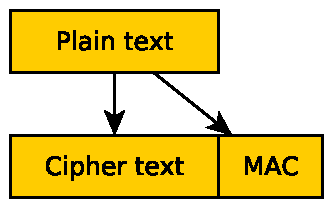
\includegraphics[width=0.9\textwidth]{images/encrypt-and-mac.pdf}
    \caption{Encrypt-and-MAC}
  \end{subfigure}
  \begin{subfigure}[b]{0.3\textwidth}
    \centering
    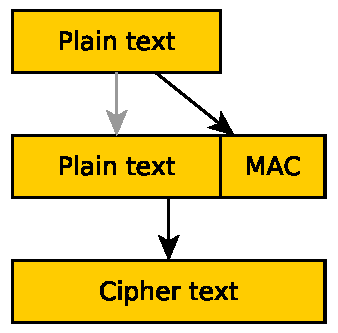
\includegraphics[width=0.9\textwidth]{images/mac-then-encrypt.pdf}
    \caption{MAC-then-encrypt}
  \end{subfigure}
  \begin{subfigure}[b]{0.3\textwidth}
    \centering
    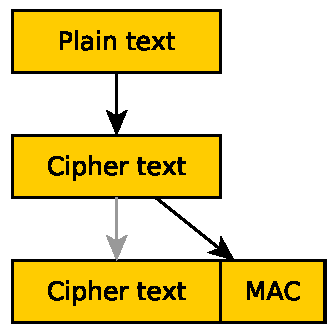
\includegraphics[width=0.9\textwidth]{images/encrypt-then-mac.pdf}
    \caption{Encrypt-then-MAC}
  \end{subfigure}
  \caption{Generic compositions of Authentized Encryption}
\end{figure}

\section{Competition for Authenticated Encryption: Security, Applicability and Robustness}

CAESAR is worldwide cryptographic competition, focused on finding new methods of authenticated encryption, that offer advantages against commonly used AES-GCM and will be suitable for widespread adoption. Submitted algorithms will be publicly evaluated by committee of researchers in fields of cryptography and cryptoanalysis.

\todo{popis algoritmů byly v soutěži, v čem se lišily, jaké a jak v nich byly nalezeny zranitelnosti a proto nepostoupily}

\todo{výběr algoritmu pro implementaci}

\subsection{Selection criteria}

\begin{description}
  \item[Online (one-pass)]
\end{description}



\subsection{NORX}

NO(T A)RX

ARX - Addition, Rotation, XOR

\subsubsection{Design goals}

\begin{itemize}
  \item \textbf{High security}
  \item \textbf{High speed} (in SW \textit{and} HW)
  \item \textbf{Simplicity} (of spec \textit{and} code)
  \item Online / one-pass
  \item Scalability (parallelism, unrolling)
  \item High key agility (no "key schedule")
  \item Side-channel leaks robustness (esp. timings)
\end{itemize}

\subsubsection{Parameters}

\begin{description}
  \item[Word Bit Size] $W \in {32, 64}$
  \item[Number of Rounds] $1 \leq R \leq 63$
  \item[Parallelism Degree] $0 \leq D \leq 255$ (0?)
  \item[Tag Bit Size] $|A| \leq 10W$
\end{description}

\begin{table}
  \centering
  \csvreader[
    after head=\begin{tabular}{llll}\toprule\csvlinetotablerow\\\midrule,
    late after line=\\,
    late after last line=\\\bottomrule\end{tabular}
  ]
    {tables/norx-proposed-instances.csv}{}
    {\texttt{\csvcoli} & \csvcolii & \csvcoliii & \csvcoliv}

  \caption{NORX proposed instances}
\end{table}

R=6: higher security margin

D=4: high throughput on parallel architectures

\subsection{Selection}

Benchmarks - Supercop, Brutus

\url{https://eprint.iacr.org/2014/850.pdf}
\url{http://www1.spms.ntu.edu.sg/~syllab/speed/}



\chapter{Implementing a new TLS cipher suite in OpenSSL}

\todo{popis částí v knihovně, které budu upravovat}

All cipher suites whose first byte is 0xFF are considered private and can be used for defining local/experimental algorithms. \cite[p.~55]{rfc2246}



\section{Creating new cipher}

\section{Creating new cipher suite}

\section{Testing}

\todo{compile a server and a client app with my edited library}
\todo{configure server to use the new cipher}
\todo{watch network traffic between them with Wireshark, confirm it is used}

All benchmarks were taken on a computer with the following configuration: CPU Intel Core i5-2540M (AES-NI, AVX capable), RAM 8 GB, OS Linux Fedora 21 (kernel 3.17.7, 64 bit).

openssl list-cipher-commands
openssl list-cipher-algorithms

openssl speed
generate cert
openssl s\_server -cert ...
openssl s\_client -connect 127.0.0.1:4433
openssl s\_time

\begin{conclusion}

  \todo{result}

\end{conclusion}

%\nocite{*}
\bibliographystyle{iso690}
\bibliography{DP_Zak_Jan_2015}

\appendix
\chapter{Acronyms}

\begin{description}
  \item[AEAD] Authenticated Encryption with Associated Data
  \item[AES] Anvanced Encryption Standard
  \item[AES-NI] Advanced Encryption Standard New Instructions
  \item[AVX] Advanced Vector Extensions
  \item[CAESAR] Competition for Authenticated Encryption: Security, Applicability and Robustness
  \item[DTLS] Datagram Transport Layer Security
  \item[IETF] Internet Engineering Task Force
  \item[ISO] International Organization for Standardization
  \item[LTS] Long Term Support
  \item[MAC] Message Authentication Code
  \item[PRF] Pseudorandom Function
  \item[RFC] Request for Comments
  \item[SSL] Secure Sockets Layer
  \item[TCP] Transmission Control Protocol
  \item[TLS] Transport Layer Security
  \item[UDP] User Datagram Protocol
\end{description}

\chapter{Content of attached CD}

\todo{obsah CD}

\begin{figure}
  \dirtree{%
    .1 readme.txt\DTcomment{the file with CD contents description}.
    .1 exe\DTcomment{the directory with executables}.
    .1 src\DTcomment{the directory of source codes}.
    .2 wbdcm\DTcomment{implementation sources}.
    .2 thesis\DTcomment{the directory of \LaTeX{} source codes of the thesis}.
    .1 text\DTcomment{the thesis text directory}.
    .2 thesis.pdf\DTcomment{the thesis text in PDF format}.
    .2 thesis.ps\DTcomment{the thesis text in PS format}.
  }
\end{figure}



\end{document}
